\documentclass{article}

\usepackage[spanish]{babel}
\usepackage[utf8]{inputenc} % Para usar tildes Unicode
\usepackage[top=0.5cm, bottom=0.5cm, left=2cm, right=2cm]{geometry}
\usepackage[colorlinks=true, urlcolor=blue]{hyperref}
\usepackage{graphicx}
\usepackage{float}

\setlength{\parindent}{1cm}

\title{Representación de curvas y árboles en 3D por medio de descriptores 1D}
\author{Ortega Ortu\~no Eder}
\date{} % Para evitar que salga la fecha al llamar a 'maketitle'

\begin{document}
	\pagenumbering{gobble} % Ocultar pagenumber
	\maketitle
	\normalsize{
La conferencia trató sobre la investigación que el Dr. Ernesto Bribiesca ha hecho para construir modelos tridimensionales mediante sencillas identidades que conforman un lenguaje gracias a las cinco o seis rotaciones que pueden tomar para así generar modelos más complejos que se fueron mostrando a lo largo de la exposición.
\\

Dicha plática comenzó con una sencilla introducción a estas entidades explicando las rotaciones de 90 que pueden tomar, lo que forma un pequeño lenguaje de entre cinco y seis elementos suficientes para aproximar el trazo de una curva. Posteriormente habló en breve sobre algunas de sus propiedades de dichos elementos tales como la reflexión que permitía básicamente lograr un efecto espejo. Todo lo anterior es lo suficiente para comenzar a generar dichos modelos matemáticos, cosa que no se hizo tan compleja de entender gracias a la notación numérica y de colores utilizada, aunque si fueron un poco confusos los ejemplos iniciales.
\\

Posteriormente nos mostró unos ejemplos de secuencias de cadenas numéricas que representaban precisamente la posición de cada entidad; con ese código era posible generar cubos cada vez más complejos hechos simplemente aprovechando las propiedades mencionadas anteriormente; todos ellos tenían en común que estaban hechos de una especie de tubos pequeñísimos por los que circulaba una esfera de inicio a fin; conforme se mostraban más ejemplos, las cadenas se hacían tremendamente largas y por ende las figuras eran mucho más complejas.
\\

Después, el Dr. Bribiesca habló sobre la generación de todas las combinaciones que se podían lograr con estas entidades y que sin duda eran demasiadas, por ello fue reconocido ya que con su equipo de investigadores logró calcular más de 200 000 con ayuda de supercomputadoras y mediante herramientas que se incluyen en el software de Autodesk AutoCAD.
\\

En la última parte de la exposición se mencionó sobre el trazado del vuelo de un avión sobre el volcán Iztaccíhuatl utilizando todo lo anterior, cosa que despertó un poco mi atención ya que con ello fue posible determinar las variaciones del terreno que sobrevoló dicho avión.
\\

Finalmente en la parte de preguntas, la profesora Miriam Pescador hizo algunas preguntas interesantes, por ejemplo sobre qué pasaría si en dichos modelos matemáticos además fuera posible incluir rotaciones de 45 o algunos otros, a lo que el profesor contestó que sin duda el lenguaje crecería considerablemente debido a la cantidad de combinaciones posibles.
\\

Para concluir el evento, el profesor Genaro Juárez y los organizadores del evento hicieron entrega de un reconocimiento al Dr. Bribiesca por su participación en Expo ESCOM 2014.
}

\begin{figure}[h]
\centering
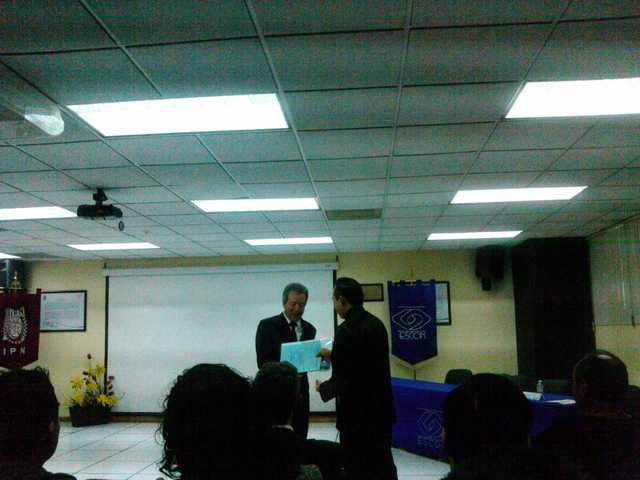
\includegraphics[width=200px]{j.jpg}
\end{figure}

\large{\hfill \textbf{Hecho en } \LaTeX - \url{multiaportes.com}}

\end{document}